\documentclass[twoside]{book}

% Packages required by doxygen
\usepackage{fixltx2e}
\usepackage{calc}
\usepackage{doxygen}
\usepackage[export]{adjustbox} % also loads graphicx
\usepackage{graphicx}
\usepackage[utf8]{inputenc}
\usepackage{makeidx}
\usepackage{multicol}
\usepackage{multirow}
\PassOptionsToPackage{warn}{textcomp}
\usepackage{textcomp}
\usepackage[nointegrals]{wasysym}
\usepackage[table]{xcolor}

% Font selection
\usepackage[T1]{fontenc}
\usepackage[scaled=.90]{helvet}
\usepackage{courier}
\usepackage{amssymb}
\usepackage{sectsty}
\renewcommand{\familydefault}{\sfdefault}
\allsectionsfont{%
  \fontseries{bc}\selectfont%
  \color{darkgray}%
}
\renewcommand{\DoxyLabelFont}{%
  \fontseries{bc}\selectfont%
  \color{darkgray}%
}
\newcommand{\+}{\discretionary{\mbox{\scriptsize$\hookleftarrow$}}{}{}}

% Page & text layout
\usepackage{geometry}
\geometry{%
  a4paper,%
  top=2.5cm,%
  bottom=2.5cm,%
  left=2.5cm,%
  right=2.5cm%
}
\tolerance=750
\hfuzz=15pt
\hbadness=750
\setlength{\emergencystretch}{15pt}
\setlength{\parindent}{0cm}
\setlength{\parskip}{3ex plus 2ex minus 2ex}
\makeatletter
\renewcommand{\paragraph}{%
  \@startsection{paragraph}{4}{0ex}{-1.0ex}{1.0ex}{%
    \normalfont\normalsize\bfseries\SS@parafont%
  }%
}
\renewcommand{\subparagraph}{%
  \@startsection{subparagraph}{5}{0ex}{-1.0ex}{1.0ex}{%
    \normalfont\normalsize\bfseries\SS@subparafont%
  }%
}
\makeatother

% Headers & footers
\usepackage{fancyhdr}
\pagestyle{fancyplain}
\fancyhead[LE]{\fancyplain{}{\bfseries\thepage}}
\fancyhead[CE]{\fancyplain{}{}}
\fancyhead[RE]{\fancyplain{}{\bfseries\leftmark}}
\fancyhead[LO]{\fancyplain{}{\bfseries\rightmark}}
\fancyhead[CO]{\fancyplain{}{}}
\fancyhead[RO]{\fancyplain{}{\bfseries\thepage}}
\fancyfoot[LE]{\fancyplain{}{}}
\fancyfoot[CE]{\fancyplain{}{}}
\fancyfoot[RE]{\fancyplain{}{\bfseries\scriptsize Generated by Doxygen }}
\fancyfoot[LO]{\fancyplain{}{\bfseries\scriptsize Generated by Doxygen }}
\fancyfoot[CO]{\fancyplain{}{}}
\fancyfoot[RO]{\fancyplain{}{}}
\renewcommand{\footrulewidth}{0.4pt}
\renewcommand{\chaptermark}[1]{%
  \markboth{#1}{}%
}
\renewcommand{\sectionmark}[1]{%
  \markright{\thesection\ #1}%
}

% Indices & bibliography
\usepackage{natbib}
\usepackage[titles]{tocloft}
\setcounter{tocdepth}{3}
\setcounter{secnumdepth}{5}
\makeindex

% Hyperlinks (required, but should be loaded last)
\usepackage{ifpdf}
\ifpdf
  \usepackage[pdftex,pagebackref=true]{hyperref}
\else
  \usepackage[ps2pdf,pagebackref=true]{hyperref}
\fi
\hypersetup{%
  colorlinks=true,%
  linkcolor=blue,%
  citecolor=blue,%
  unicode%
}

% Custom commands
\newcommand{\clearemptydoublepage}{%
  \newpage{\pagestyle{empty}\cleardoublepage}%
}

\usepackage{caption}
\captionsetup{labelsep=space,justification=centering,font={bf},singlelinecheck=off,skip=4pt,position=top}

%===== C O N T E N T S =====

\begin{document}

% Titlepage & ToC
\hypersetup{pageanchor=false,
             bookmarksnumbered=true,
             pdfencoding=unicode
            }
\pagenumbering{alph}
\begin{titlepage}
\vspace*{7cm}
\begin{center}%
{\Large Graphics Engine \\[1ex]\large 1.\+0 }\\
\vspace*{1cm}
{\large Generated by Doxygen 1.8.14}\\
\end{center}
\end{titlepage}
\clearemptydoublepage
\pagenumbering{roman}
\tableofcontents
\clearemptydoublepage
\pagenumbering{arabic}
\hypersetup{pageanchor=true}

%--- Begin generated contents ---
\chapter{3802\+I\+CT}
\label{md__r_e_a_d_m_e}
\Hypertarget{md__r_e_a_d_m_e}
\input{md__r_e_a_d_m_e}
\chapter{Class Index}
\section{Class List}
Here are the classes, structs, unions and interfaces with brief descriptions\+:\begin{DoxyCompactList}
\item\contentsline{section}{\mbox{\hyperlink{structcolour}{colour}} }{\pageref{structcolour}}{}
\item\contentsline{section}{\mbox{\hyperlink{classmatrix}{matrix}} }{\pageref{classmatrix}}{}
\item\contentsline{section}{\mbox{\hyperlink{structpoint}{point}} }{\pageref{structpoint}}{}
\item\contentsline{section}{\mbox{\hyperlink{class_polygon}{Polygon}} }{\pageref{class_polygon}}{}
\item\contentsline{section}{\mbox{\hyperlink{structrectangle}{rectangle}} }{\pageref{structrectangle}}{}
\item\contentsline{section}{\mbox{\hyperlink{class_text}{Text}} }{\pageref{class_text}}{}
\item\contentsline{section}{\mbox{\hyperlink{structvelocity}{velocity}} }{\pageref{structvelocity}}{}
\end{DoxyCompactList}

\chapter{Class Documentation}
\hypertarget{structcolour}{}\section{colour Struct Reference}
\label{structcolour}\index{colour@{colour}}


{\ttfamily \#include $<$structs.\+h$>$}

\subsection*{Public Attributes}
\begin{DoxyCompactItemize}
\item 
\mbox{\Hypertarget{structcolour_af66bc24a6bed26fe8d97cb512caa97de}\label{structcolour_af66bc24a6bed26fe8d97cb512caa97de}} 
double {\bfseries R}
\item 
\mbox{\Hypertarget{structcolour_ae459b0b040ebe7eb15e77b26760ac53a}\label{structcolour_ae459b0b040ebe7eb15e77b26760ac53a}} 
double {\bfseries G}
\item 
\mbox{\Hypertarget{structcolour_ab8699c79e9d979c413799dcf47e606d2}\label{structcolour_ab8699c79e9d979c413799dcf47e606d2}} 
double {\bfseries B}
\end{DoxyCompactItemize}


\subsection{Detailed Description}
Three doubles representing values for red, green and blue respectively 
\begin{DoxyParams}{Parameters}
{\em R} & red value \\
\hline
{\em G} & green value \\
\hline
{\em B} & blue value \\
\hline
\end{DoxyParams}


The documentation for this struct was generated from the following file\+:\begin{DoxyCompactItemize}
\item 
structs.\+h\end{DoxyCompactItemize}

\hypertarget{classmatrix}{}\section{matrix Class Reference}
\label{classmatrix}\index{matrix@{matrix}}
\subsection*{Public Member Functions}
\begin{DoxyCompactItemize}
\item 
\mbox{\hyperlink{classmatrix_a2994d419451e97702e5b1cc12c81d914}{matrix}} (int num\+\_\+rows, int num\+\_\+cols)
\item 
\mbox{\hyperlink{classmatrix_a4daf70b1506ea976352f20e4322a9c17}{matrix}} ()
\item 
void \mbox{\hyperlink{classmatrix_a2e865089f895c8a84c37818cf75ca215}{set\+\_\+row}} (int row\+\_\+number, std\+::vector$<$ double $>$ row)
\item 
void \mbox{\hyperlink{classmatrix_a976c7dba1c9f40d6c129067fd4c5afc1}{set\+\_\+col}} (int col\+\_\+number, std\+::vector$<$ double $>$ col)
\item 
void \mbox{\hyperlink{classmatrix_a761067e4f67f5b9c23594cbc1d8ce696}{set\+\_\+val}} (int row\+\_\+number, int col\+\_\+number, double val)
\item 
void \mbox{\hyperlink{classmatrix_ae9817c7c1a8855874728c2342f514885}{add\+\_\+val}} (int row\+\_\+number, int col\+\_\+number, double val)
\item 
double \mbox{\hyperlink{classmatrix_a4913d355d918c769b200cc0b6bffbd68}{get\+\_\+val}} (int row\+\_\+number, int col\+\_\+number)
\item 
int \mbox{\hyperlink{classmatrix_a528d089b9734f7cda64ffab3a2d2831f}{get\+\_\+rows}} ()
\item 
int \mbox{\hyperlink{classmatrix_ae8479003bb1373c0f27f7f59980d5e3a}{get\+\_\+cols}} ()
\item 
void \mbox{\hyperlink{classmatrix_a820379d929b5a1c49c9df0d05f91c7e2}{print}} ()
\item 
\mbox{\hyperlink{classmatrix}{matrix}} \mbox{\hyperlink{classmatrix_a34563095940d2be0e50d98fbb2ba9ead}{multiply}} (\mbox{\hyperlink{classmatrix}{matrix}} other\+\_\+matrix)
\item 
void \mbox{\hyperlink{classmatrix_a159c12c74a7a58596e297a29094eb1f9}{set\+\_\+up\+\_\+transformation}} ()
\end{DoxyCompactItemize}


\subsection{Constructor \& Destructor Documentation}
\mbox{\Hypertarget{classmatrix_a2994d419451e97702e5b1cc12c81d914}\label{classmatrix_a2994d419451e97702e5b1cc12c81d914}} 
\index{matrix@{matrix}!matrix@{matrix}}
\index{matrix@{matrix}!matrix@{matrix}}
\subsubsection{\texorpdfstring{matrix()}{matrix()}\hspace{0.1cm}{\footnotesize\ttfamily [1/2]}}
{\footnotesize\ttfamily matrix\+::matrix (\begin{DoxyParamCaption}\item[{int}]{rows,  }\item[{int}]{cols }\end{DoxyParamCaption})}

Constructor for a matrix when given and number of rows and columns 
\begin{DoxyParams}{Parameters}
{\em rows} & an integer representing the number of rows the matrix should have \\
\hline
{\em cols} & an integer representing the number of columns the matrix should have \\
\hline
\end{DoxyParams}
\mbox{\Hypertarget{classmatrix_a4daf70b1506ea976352f20e4322a9c17}\label{classmatrix_a4daf70b1506ea976352f20e4322a9c17}} 
\index{matrix@{matrix}!matrix@{matrix}}
\index{matrix@{matrix}!matrix@{matrix}}
\subsubsection{\texorpdfstring{matrix()}{matrix()}\hspace{0.1cm}{\footnotesize\ttfamily [2/2]}}
{\footnotesize\ttfamily matrix\+::matrix (\begin{DoxyParamCaption}{ }\end{DoxyParamCaption})}

Constructor for a matrix if not given a size. Makes a 4 by 4 matrix 

\subsection{Member Function Documentation}
\mbox{\Hypertarget{classmatrix_ae9817c7c1a8855874728c2342f514885}\label{classmatrix_ae9817c7c1a8855874728c2342f514885}} 
\index{matrix@{matrix}!add\+\_\+val@{add\+\_\+val}}
\index{add\+\_\+val@{add\+\_\+val}!matrix@{matrix}}
\subsubsection{\texorpdfstring{add\+\_\+val()}{add\_val()}}
{\footnotesize\ttfamily void matrix\+::add\+\_\+val (\begin{DoxyParamCaption}\item[{int}]{row\+\_\+number,  }\item[{int}]{col\+\_\+number,  }\item[{double}]{val }\end{DoxyParamCaption})}

Adds a value at the given row and column with the given value 
\begin{DoxyParams}{Parameters}
{\em row\+\_\+number} & integer representing which row to replace \\
\hline
{\em col\+\_\+number} & integer representing which column to replace \\
\hline
{\em val} & double representing the value to add in the matrix \\
\hline
\end{DoxyParams}
\mbox{\Hypertarget{classmatrix_ae8479003bb1373c0f27f7f59980d5e3a}\label{classmatrix_ae8479003bb1373c0f27f7f59980d5e3a}} 
\index{matrix@{matrix}!get\+\_\+cols@{get\+\_\+cols}}
\index{get\+\_\+cols@{get\+\_\+cols}!matrix@{matrix}}
\subsubsection{\texorpdfstring{get\+\_\+cols()}{get\_cols()}}
{\footnotesize\ttfamily int matrix\+::get\+\_\+cols (\begin{DoxyParamCaption}{ }\end{DoxyParamCaption})}

Returns the number of columns the matrix has \mbox{\Hypertarget{classmatrix_a528d089b9734f7cda64ffab3a2d2831f}\label{classmatrix_a528d089b9734f7cda64ffab3a2d2831f}} 
\index{matrix@{matrix}!get\+\_\+rows@{get\+\_\+rows}}
\index{get\+\_\+rows@{get\+\_\+rows}!matrix@{matrix}}
\subsubsection{\texorpdfstring{get\+\_\+rows()}{get\_rows()}}
{\footnotesize\ttfamily int matrix\+::get\+\_\+rows (\begin{DoxyParamCaption}{ }\end{DoxyParamCaption})}

Returns the number of rows the matrix has \mbox{\Hypertarget{classmatrix_a4913d355d918c769b200cc0b6bffbd68}\label{classmatrix_a4913d355d918c769b200cc0b6bffbd68}} 
\index{matrix@{matrix}!get\+\_\+val@{get\+\_\+val}}
\index{get\+\_\+val@{get\+\_\+val}!matrix@{matrix}}
\subsubsection{\texorpdfstring{get\+\_\+val()}{get\_val()}}
{\footnotesize\ttfamily double matrix\+::get\+\_\+val (\begin{DoxyParamCaption}\item[{int}]{row\+\_\+number,  }\item[{int}]{col\+\_\+number }\end{DoxyParamCaption})}

Returns a value at the given row and column 
\begin{DoxyParams}{Parameters}
{\em row\+\_\+number} & integer representing which row to replace \\
\hline
{\em col\+\_\+number} & integer representing which column to replace \\
\hline
\end{DoxyParams}
\mbox{\Hypertarget{classmatrix_a34563095940d2be0e50d98fbb2ba9ead}\label{classmatrix_a34563095940d2be0e50d98fbb2ba9ead}} 
\index{matrix@{matrix}!multiply@{multiply}}
\index{multiply@{multiply}!matrix@{matrix}}
\subsubsection{\texorpdfstring{multiply()}{multiply()}}
{\footnotesize\ttfamily \mbox{\hyperlink{classmatrix}{matrix}} matrix\+::multiply (\begin{DoxyParamCaption}\item[{\mbox{\hyperlink{classmatrix}{matrix}}}]{other\+\_\+matrix }\end{DoxyParamCaption})}

Performs matrix dot multiplication between this matrix and a given matrix 
\begin{DoxyParams}{Parameters}
{\em other\+\_\+matrix} & the matrix to multiply with \\
\hline
\end{DoxyParams}
\mbox{\Hypertarget{classmatrix_a820379d929b5a1c49c9df0d05f91c7e2}\label{classmatrix_a820379d929b5a1c49c9df0d05f91c7e2}} 
\index{matrix@{matrix}!print@{print}}
\index{print@{print}!matrix@{matrix}}
\subsubsection{\texorpdfstring{print()}{print()}}
{\footnotesize\ttfamily void matrix\+::print (\begin{DoxyParamCaption}{ }\end{DoxyParamCaption})}

Prints out the matrix to stdout in a formatted way \mbox{\Hypertarget{classmatrix_a976c7dba1c9f40d6c129067fd4c5afc1}\label{classmatrix_a976c7dba1c9f40d6c129067fd4c5afc1}} 
\index{matrix@{matrix}!set\+\_\+col@{set\+\_\+col}}
\index{set\+\_\+col@{set\+\_\+col}!matrix@{matrix}}
\subsubsection{\texorpdfstring{set\+\_\+col()}{set\_col()}}
{\footnotesize\ttfamily void matrix\+::set\+\_\+col (\begin{DoxyParamCaption}\item[{int}]{col\+\_\+number,  }\item[{std\+::vector$<$ double $>$}]{col }\end{DoxyParamCaption})}

Replaces a col in the matrix with the given vector 
\begin{DoxyParams}{Parameters}
{\em col\+\_\+number} & integer representing which column to replace \\
\hline
{\em col} & vector of doubles representing the new col values \\
\hline
\end{DoxyParams}
\mbox{\Hypertarget{classmatrix_a2e865089f895c8a84c37818cf75ca215}\label{classmatrix_a2e865089f895c8a84c37818cf75ca215}} 
\index{matrix@{matrix}!set\+\_\+row@{set\+\_\+row}}
\index{set\+\_\+row@{set\+\_\+row}!matrix@{matrix}}
\subsubsection{\texorpdfstring{set\+\_\+row()}{set\_row()}}
{\footnotesize\ttfamily void matrix\+::set\+\_\+row (\begin{DoxyParamCaption}\item[{int}]{row\+\_\+number,  }\item[{std\+::vector$<$ double $>$}]{row }\end{DoxyParamCaption})}

Replaces a row in the matrix with the given vector 
\begin{DoxyParams}{Parameters}
{\em row\+\_\+number} & integer representing which row to replace \\
\hline
{\em row} & vector of doubles representing the new row values \\
\hline
\end{DoxyParams}
\mbox{\Hypertarget{classmatrix_a159c12c74a7a58596e297a29094eb1f9}\label{classmatrix_a159c12c74a7a58596e297a29094eb1f9}} 
\index{matrix@{matrix}!set\+\_\+up\+\_\+transformation@{set\+\_\+up\+\_\+transformation}}
\index{set\+\_\+up\+\_\+transformation@{set\+\_\+up\+\_\+transformation}!matrix@{matrix}}
\subsubsection{\texorpdfstring{set\+\_\+up\+\_\+transformation()}{set\_up\_transformation()}}
{\footnotesize\ttfamily void matrix\+::set\+\_\+up\+\_\+transformation (\begin{DoxyParamCaption}{ }\end{DoxyParamCaption})}

Sets up the matrix as a blank transformation matrix \mbox{\Hypertarget{classmatrix_a761067e4f67f5b9c23594cbc1d8ce696}\label{classmatrix_a761067e4f67f5b9c23594cbc1d8ce696}} 
\index{matrix@{matrix}!set\+\_\+val@{set\+\_\+val}}
\index{set\+\_\+val@{set\+\_\+val}!matrix@{matrix}}
\subsubsection{\texorpdfstring{set\+\_\+val()}{set\_val()}}
{\footnotesize\ttfamily void matrix\+::set\+\_\+val (\begin{DoxyParamCaption}\item[{int}]{row\+\_\+number,  }\item[{int}]{col\+\_\+number,  }\item[{double}]{val }\end{DoxyParamCaption})}

Replaces a value at the given row and column with the given value 
\begin{DoxyParams}{Parameters}
{\em row\+\_\+number} & integer representing which row to replace \\
\hline
{\em col\+\_\+number} & integer representing which column to replace \\
\hline
{\em val} & double representing the value to use in the matrix \\
\hline
\end{DoxyParams}


The documentation for this class was generated from the following files\+:\begin{DoxyCompactItemize}
\item 
matrix.\+h\item 
matrix.\+cpp\end{DoxyCompactItemize}

\hypertarget{structpoint}{}\section{point Struct Reference}
\label{structpoint}\index{point@{point}}


{\ttfamily \#include $<$structs.\+h$>$}

\subsection*{Public Attributes}
\begin{DoxyCompactItemize}
\item 
\mbox{\Hypertarget{structpoint_ad679b07fb69d55f5ad454d0f1f2891d5}\label{structpoint_ad679b07fb69d55f5ad454d0f1f2891d5}} 
int {\bfseries x}
\item 
\mbox{\Hypertarget{structpoint_a9a82ca9504acabb1e30569f89c805471}\label{structpoint_a9a82ca9504acabb1e30569f89c805471}} 
int {\bfseries y}
\end{DoxyCompactItemize}


\subsection{Detailed Description}
Two integers representing a pixel on the screen 
\begin{DoxyParams}{Parameters}
{\em x} & x co-\/ordinate of pixel \\
\hline
{\em y} & y co-\/ordinate of pixel \\
\hline
\end{DoxyParams}


The documentation for this struct was generated from the following file\+:\begin{DoxyCompactItemize}
\item 
structs.\+h\end{DoxyCompactItemize}

\hypertarget{class_polygon}{}\section{Polygon Class Reference}
\label{class_polygon}\index{Polygon@{Polygon}}
\subsection*{Public Member Functions}
\begin{DoxyCompactItemize}
\item 
\mbox{\hyperlink{class_polygon_a7c9801ab8183848cda1a9e4e355973cc}{Polygon}} (std\+::vector$<$ \mbox{\hyperlink{structpoint}{point}} $>$ points, \mbox{\hyperlink{structpoint}{point}} coordinates)
\item 
\mbox{\hyperlink{class_polygon_a84c5ba9b7d4fbbfd85e2485712d282d8}{Polygon}} (std\+::vector$<$ \mbox{\hyperlink{structpoint}{point}} $>$ points)
\item 
\mbox{\hyperlink{class_polygon_ac183e712f8be1e13f1c9d5b4d4512ead}{Polygon}} ()
\item 
void \mbox{\hyperlink{class_polygon_ab5a643b45071142291a93070f36e9159}{change\+\_\+points}} (std\+::vector$<$ \mbox{\hyperlink{structpoint}{point}} $>$ points)
\item 
void \mbox{\hyperlink{class_polygon_a5895893a117ad4fba5422e9269ff729c}{set\+\_\+colour}} (\mbox{\hyperlink{structcolour}{colour}} R\+GB)
\item 
void \mbox{\hyperlink{class_polygon_a17428a7d7dff4653c905b91020a9f803}{draw}} ()
\item 
void \mbox{\hyperlink{class_polygon_a3166ec344b0453bde49f6c32300eab12}{scale}} (int x\+\_\+scale, int y\+\_\+scale)
\item 
void \mbox{\hyperlink{class_polygon_ae5993bb89530d873701d9d5558494c09}{rotate}} (double angle)
\item 
void \mbox{\hyperlink{class_polygon_aa058b0c05dcb8a9c4c0f2737ac59fb64}{additive\+\_\+rotate}} (double angle)
\item 
void \mbox{\hyperlink{class_polygon_a8981ae2ebe960a7355134f03dc88f1e3}{translate}} (double x\+\_\+offset, double y\+\_\+offset)
\item 
void \mbox{\hyperlink{class_polygon_aa066ce6c55fe73f2187919085016e9ec}{additive\+\_\+translate}} (double x\+\_\+offset, double y\+\_\+offset)
\item 
void \mbox{\hyperlink{class_polygon_aca723d97ae607e5079cd5dfd7ba616d3}{save\+\_\+transformation}} ()
\item 
void \mbox{\hyperlink{class_polygon_a9c058c0a82c8d8138301d2c6ec049d09}{undo\+\_\+transformation}} ()
\item 
\mbox{\hyperlink{structpoint}{point}} \mbox{\hyperlink{class_polygon_a1c99b0b80833ef2eca19b98530d90910}{find\+\_\+top\+\_\+left\+\_\+point}} ()
\item 
\mbox{\hyperlink{structpoint}{point}} \mbox{\hyperlink{class_polygon_a1f9b4d001197e6ff84fb4ed50b47be59}{find\+\_\+bottom\+\_\+right\+\_\+point}} ()
\end{DoxyCompactItemize}


\subsection{Constructor \& Destructor Documentation}
\mbox{\Hypertarget{class_polygon_a7c9801ab8183848cda1a9e4e355973cc}\label{class_polygon_a7c9801ab8183848cda1a9e4e355973cc}} 
\index{Polygon@{Polygon}!Polygon@{Polygon}}
\index{Polygon@{Polygon}!Polygon@{Polygon}}
\subsubsection{\texorpdfstring{Polygon()}{Polygon()}\hspace{0.1cm}{\footnotesize\ttfamily [1/3]}}
{\footnotesize\ttfamily Polygon\+::\+Polygon (\begin{DoxyParamCaption}\item[{std\+::vector$<$ \mbox{\hyperlink{structpoint}{point}} $>$}]{points,  }\item[{\mbox{\hyperlink{structpoint}{point}}}]{coordinates }\end{DoxyParamCaption})}

Constructor for a polygon when give the points and a starting point 
\begin{DoxyParams}{Parameters}
{\em points} & vector of points representing the points making up the polygon \\
\hline
{\em coordinates} & a point representing where the polygon should be drawn on the screen \\
\hline
\end{DoxyParams}
\mbox{\Hypertarget{class_polygon_a84c5ba9b7d4fbbfd85e2485712d282d8}\label{class_polygon_a84c5ba9b7d4fbbfd85e2485712d282d8}} 
\index{Polygon@{Polygon}!Polygon@{Polygon}}
\index{Polygon@{Polygon}!Polygon@{Polygon}}
\subsubsection{\texorpdfstring{Polygon()}{Polygon()}\hspace{0.1cm}{\footnotesize\ttfamily [2/3]}}
{\footnotesize\ttfamily Polygon\+::\+Polygon (\begin{DoxyParamCaption}\item[{std\+::vector$<$ \mbox{\hyperlink{structpoint}{point}} $>$}]{points }\end{DoxyParamCaption})}

Constructor for a polygon when give the points. Draws the polygon at 0, 0 
\begin{DoxyParams}{Parameters}
{\em points} & vector of points representing the points making up the polygon \\
\hline
\end{DoxyParams}
\mbox{\Hypertarget{class_polygon_ac183e712f8be1e13f1c9d5b4d4512ead}\label{class_polygon_ac183e712f8be1e13f1c9d5b4d4512ead}} 
\index{Polygon@{Polygon}!Polygon@{Polygon}}
\index{Polygon@{Polygon}!Polygon@{Polygon}}
\subsubsection{\texorpdfstring{Polygon()}{Polygon()}\hspace{0.1cm}{\footnotesize\ttfamily [3/3]}}
{\footnotesize\ttfamily Polygon\+::\+Polygon (\begin{DoxyParamCaption}{ }\end{DoxyParamCaption})}

Constructor for a blank \mbox{\hyperlink{class_polygon}{Polygon}}. Defines one point at 0, 0 and draws it at 0, 0 

\subsection{Member Function Documentation}
\mbox{\Hypertarget{class_polygon_aa058b0c05dcb8a9c4c0f2737ac59fb64}\label{class_polygon_aa058b0c05dcb8a9c4c0f2737ac59fb64}} 
\index{Polygon@{Polygon}!additive\+\_\+rotate@{additive\+\_\+rotate}}
\index{additive\+\_\+rotate@{additive\+\_\+rotate}!Polygon@{Polygon}}
\subsubsection{\texorpdfstring{additive\+\_\+rotate()}{additive\_rotate()}}
{\footnotesize\ttfamily void Polygon\+::additive\+\_\+rotate (\begin{DoxyParamCaption}\item[{double}]{angle }\end{DoxyParamCaption})}

Rotates the \mbox{\hyperlink{class_polygon}{Polygon}} by the given angle (Adds to rotation) 
\begin{DoxyParams}{Parameters}
{\em angle} & double representing the angle in degrees \\
\hline
\end{DoxyParams}
\mbox{\Hypertarget{class_polygon_aa066ce6c55fe73f2187919085016e9ec}\label{class_polygon_aa066ce6c55fe73f2187919085016e9ec}} 
\index{Polygon@{Polygon}!additive\+\_\+translate@{additive\+\_\+translate}}
\index{additive\+\_\+translate@{additive\+\_\+translate}!Polygon@{Polygon}}
\subsubsection{\texorpdfstring{additive\+\_\+translate()}{additive\_translate()}}
{\footnotesize\ttfamily void Polygon\+::additive\+\_\+translate (\begin{DoxyParamCaption}\item[{double}]{x\+\_\+offset,  }\item[{double}]{y\+\_\+offset }\end{DoxyParamCaption})}

Translates the \mbox{\hyperlink{class_polygon}{Polygon}} by the given dimensions (Adds to translation) 
\begin{DoxyParams}{Parameters}
{\em x\+\_\+scale} & integer representing what to move the x value of the \mbox{\hyperlink{class_polygon}{Polygon}} by \\
\hline
{\em y\+\_\+scale} & integer representing what to move the y value of the \mbox{\hyperlink{class_polygon}{Polygon}} by \\
\hline
\end{DoxyParams}
\mbox{\Hypertarget{class_polygon_ab5a643b45071142291a93070f36e9159}\label{class_polygon_ab5a643b45071142291a93070f36e9159}} 
\index{Polygon@{Polygon}!change\+\_\+points@{change\+\_\+points}}
\index{change\+\_\+points@{change\+\_\+points}!Polygon@{Polygon}}
\subsubsection{\texorpdfstring{change\+\_\+points()}{change\_points()}}
{\footnotesize\ttfamily void Polygon\+::change\+\_\+points (\begin{DoxyParamCaption}\item[{std\+::vector$<$ \mbox{\hyperlink{structpoint}{point}} $>$}]{points }\end{DoxyParamCaption})}

Replaces the vector the \mbox{\hyperlink{class_polygon}{Polygon}}\textquotesingle{}s points with the given vector 
\begin{DoxyParams}{Parameters}
{\em points} & vector of points representing the points making up the polygon \\
\hline
\end{DoxyParams}
\mbox{\Hypertarget{class_polygon_a17428a7d7dff4653c905b91020a9f803}\label{class_polygon_a17428a7d7dff4653c905b91020a9f803}} 
\index{Polygon@{Polygon}!draw@{draw}}
\index{draw@{draw}!Polygon@{Polygon}}
\subsubsection{\texorpdfstring{draw()}{draw()}}
{\footnotesize\ttfamily void Polygon\+::draw (\begin{DoxyParamCaption}{ }\end{DoxyParamCaption})}

Draws the \mbox{\hyperlink{class_polygon}{Polygon}} on the screen \mbox{\Hypertarget{class_polygon_a1f9b4d001197e6ff84fb4ed50b47be59}\label{class_polygon_a1f9b4d001197e6ff84fb4ed50b47be59}} 
\index{Polygon@{Polygon}!find\+\_\+bottom\+\_\+right\+\_\+point@{find\+\_\+bottom\+\_\+right\+\_\+point}}
\index{find\+\_\+bottom\+\_\+right\+\_\+point@{find\+\_\+bottom\+\_\+right\+\_\+point}!Polygon@{Polygon}}
\subsubsection{\texorpdfstring{find\+\_\+bottom\+\_\+right\+\_\+point()}{find\_bottom\_right\_point()}}
{\footnotesize\ttfamily \mbox{\hyperlink{structpoint}{point}} Polygon\+::find\+\_\+bottom\+\_\+right\+\_\+point (\begin{DoxyParamCaption}{ }\end{DoxyParamCaption})}

Finds the highest x value and the smallest y value \mbox{\Hypertarget{class_polygon_a1c99b0b80833ef2eca19b98530d90910}\label{class_polygon_a1c99b0b80833ef2eca19b98530d90910}} 
\index{Polygon@{Polygon}!find\+\_\+top\+\_\+left\+\_\+point@{find\+\_\+top\+\_\+left\+\_\+point}}
\index{find\+\_\+top\+\_\+left\+\_\+point@{find\+\_\+top\+\_\+left\+\_\+point}!Polygon@{Polygon}}
\subsubsection{\texorpdfstring{find\+\_\+top\+\_\+left\+\_\+point()}{find\_top\_left\_point()}}
{\footnotesize\ttfamily \mbox{\hyperlink{structpoint}{point}} Polygon\+::find\+\_\+top\+\_\+left\+\_\+point (\begin{DoxyParamCaption}{ }\end{DoxyParamCaption})}

Finds the smallest x value and the highest y value \mbox{\Hypertarget{class_polygon_ae5993bb89530d873701d9d5558494c09}\label{class_polygon_ae5993bb89530d873701d9d5558494c09}} 
\index{Polygon@{Polygon}!rotate@{rotate}}
\index{rotate@{rotate}!Polygon@{Polygon}}
\subsubsection{\texorpdfstring{rotate()}{rotate()}}
{\footnotesize\ttfamily void Polygon\+::rotate (\begin{DoxyParamCaption}\item[{double}]{angle }\end{DoxyParamCaption})}

Rotates the \mbox{\hyperlink{class_polygon}{Polygon}} to the given angle 
\begin{DoxyParams}{Parameters}
{\em angle} & double representing the angle in degrees \\
\hline
\end{DoxyParams}
\mbox{\Hypertarget{class_polygon_aca723d97ae607e5079cd5dfd7ba616d3}\label{class_polygon_aca723d97ae607e5079cd5dfd7ba616d3}} 
\index{Polygon@{Polygon}!save\+\_\+transformation@{save\+\_\+transformation}}
\index{save\+\_\+transformation@{save\+\_\+transformation}!Polygon@{Polygon}}
\subsubsection{\texorpdfstring{save\+\_\+transformation()}{save\_transformation()}}
{\footnotesize\ttfamily void Polygon\+::save\+\_\+transformation (\begin{DoxyParamCaption}{ }\end{DoxyParamCaption})}

Saves the currently used matrix to a stack \mbox{\Hypertarget{class_polygon_a3166ec344b0453bde49f6c32300eab12}\label{class_polygon_a3166ec344b0453bde49f6c32300eab12}} 
\index{Polygon@{Polygon}!scale@{scale}}
\index{scale@{scale}!Polygon@{Polygon}}
\subsubsection{\texorpdfstring{scale()}{scale()}}
{\footnotesize\ttfamily void Polygon\+::scale (\begin{DoxyParamCaption}\item[{int}]{x\+\_\+scale,  }\item[{int}]{y\+\_\+scale }\end{DoxyParamCaption})}

Scales the \mbox{\hyperlink{class_polygon}{Polygon}} by the given dimensions 
\begin{DoxyParams}{Parameters}
{\em x\+\_\+scale} & integer representing what to multiply the x scale of the \mbox{\hyperlink{class_polygon}{Polygon}} by \\
\hline
{\em y\+\_\+scale} & integer representing what to multiply the y scale of the \mbox{\hyperlink{class_polygon}{Polygon}} by \\
\hline
\end{DoxyParams}
\mbox{\Hypertarget{class_polygon_a5895893a117ad4fba5422e9269ff729c}\label{class_polygon_a5895893a117ad4fba5422e9269ff729c}} 
\index{Polygon@{Polygon}!set\+\_\+colour@{set\+\_\+colour}}
\index{set\+\_\+colour@{set\+\_\+colour}!Polygon@{Polygon}}
\subsubsection{\texorpdfstring{set\+\_\+colour()}{set\_colour()}}
{\footnotesize\ttfamily void Polygon\+::set\+\_\+colour (\begin{DoxyParamCaption}\item[{\mbox{\hyperlink{structcolour}{colour}}}]{R\+GB }\end{DoxyParamCaption})}

Replaces the colour the \mbox{\hyperlink{class_polygon}{Polygon}} is filled with with the given colour 
\begin{DoxyParams}{Parameters}
{\em R\+GB} & struct representing the 3 double values for R, G and B \\
\hline
\end{DoxyParams}
\mbox{\Hypertarget{class_polygon_a8981ae2ebe960a7355134f03dc88f1e3}\label{class_polygon_a8981ae2ebe960a7355134f03dc88f1e3}} 
\index{Polygon@{Polygon}!translate@{translate}}
\index{translate@{translate}!Polygon@{Polygon}}
\subsubsection{\texorpdfstring{translate()}{translate()}}
{\footnotesize\ttfamily void Polygon\+::translate (\begin{DoxyParamCaption}\item[{double}]{x\+\_\+offset,  }\item[{double}]{y\+\_\+offset }\end{DoxyParamCaption})}

Translates the \mbox{\hyperlink{class_polygon}{Polygon}} to the given dimensions 
\begin{DoxyParams}{Parameters}
{\em x\+\_\+scale} & integer representing where to move the x value of the \mbox{\hyperlink{class_polygon}{Polygon}} to \\
\hline
{\em y\+\_\+scale} & integer representing where to move the y value of the \mbox{\hyperlink{class_polygon}{Polygon}} to \\
\hline
\end{DoxyParams}
\mbox{\Hypertarget{class_polygon_a9c058c0a82c8d8138301d2c6ec049d09}\label{class_polygon_a9c058c0a82c8d8138301d2c6ec049d09}} 
\index{Polygon@{Polygon}!undo\+\_\+transformation@{undo\+\_\+transformation}}
\index{undo\+\_\+transformation@{undo\+\_\+transformation}!Polygon@{Polygon}}
\subsubsection{\texorpdfstring{undo\+\_\+transformation()}{undo\_transformation()}}
{\footnotesize\ttfamily void Polygon\+::undo\+\_\+transformation (\begin{DoxyParamCaption}{ }\end{DoxyParamCaption})}

Reverts the transformation matrix to the last saved matrix 

The documentation for this class was generated from the following files\+:\begin{DoxyCompactItemize}
\item 
polygon.\+h\item 
polygon.\+cpp\end{DoxyCompactItemize}

\hypertarget{structrectangle}{}\section{rectangle Struct Reference}
\label{structrectangle}\index{rectangle@{rectangle}}


{\ttfamily \#include $<$structs.\+h$>$}



Collaboration diagram for rectangle\+:\nopagebreak
\begin{figure}[H]
\begin{center}
\leavevmode
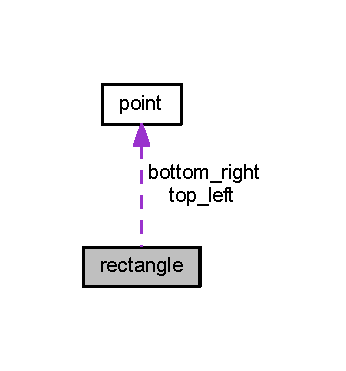
\includegraphics[width=166pt]{structrectangle__coll__graph}
\end{center}
\end{figure}
\subsection*{Public Attributes}
\begin{DoxyCompactItemize}
\item 
\mbox{\Hypertarget{structrectangle_a728703fcf5a71a4e1b156cfc6f4504e0}\label{structrectangle_a728703fcf5a71a4e1b156cfc6f4504e0}} 
\mbox{\hyperlink{structpoint}{point}} {\bfseries top\+\_\+left}
\item 
\mbox{\Hypertarget{structrectangle_a6920a2662992d3f86825dbcbe8264659}\label{structrectangle_a6920a2662992d3f86825dbcbe8264659}} 
\mbox{\hyperlink{structpoint}{point}} {\bfseries bottom\+\_\+right}
\end{DoxyCompactItemize}


\subsection{Detailed Description}
Two points representing the top left and bottom right corners to form a rectangle 
\begin{DoxyParams}{Parameters}
{\em top\+\_\+left} & point where the top left of the rectangle is located \\
\hline
{\em bottom\+\_\+right} & point where the bottom right of the recatngle is located \\
\hline
\end{DoxyParams}


The documentation for this struct was generated from the following file\+:\begin{DoxyCompactItemize}
\item 
structs.\+h\end{DoxyCompactItemize}

\hypertarget{class_text}{}\section{Text Class Reference}
\label{class_text}\index{Text@{Text}}
\subsection*{Public Member Functions}
\begin{DoxyCompactItemize}
\item 
\mbox{\hyperlink{class_text_a98ff94dc4040712884de7d62c04967d1}{Text}} (std\+::string text\+\_\+to\+\_\+display, \mbox{\hyperlink{structpoint}{point}} bottom\+\_\+left\+\_\+position, \mbox{\hyperlink{structcolour}{colour}} R\+BG)
\item 
void \mbox{\hyperlink{class_text_adedc069a9ad622bf9d2cf6d194a01b39}{draw}} ()
\item 
void \mbox{\hyperlink{class_text_ae3fc12110b4324c661aa3d279d71159c}{update\+\_\+text}} (std\+::string text\+\_\+to\+\_\+display)
\end{DoxyCompactItemize}


\subsection{Constructor \& Destructor Documentation}
\mbox{\Hypertarget{class_text_a98ff94dc4040712884de7d62c04967d1}\label{class_text_a98ff94dc4040712884de7d62c04967d1}} 
\index{Text@{Text}!Text@{Text}}
\index{Text@{Text}!Text@{Text}}
\subsubsection{\texorpdfstring{Text()}{Text()}}
{\footnotesize\ttfamily Text\+::\+Text (\begin{DoxyParamCaption}\item[{std\+::string}]{text\+\_\+to\+\_\+display,  }\item[{\mbox{\hyperlink{structpoint}{point}}}]{bottom\+\_\+left\+\_\+position,  }\item[{\mbox{\hyperlink{structcolour}{colour}}}]{R\+GB }\end{DoxyParamCaption})}

Constructor for text. Currently only supports numbers 
\begin{DoxyParams}{Parameters}
{\em text\+\_\+to\+\_\+display} & a string representing what text to display \\
\hline
{\em bottom\+\_\+left\+\_\+position} & a point representing the bottom left position to draw the text \\
\hline
{\em R\+GB} & a struct representing the R\+GB values of the colour to draw the text as \\
\hline
\end{DoxyParams}


\subsection{Member Function Documentation}
\mbox{\Hypertarget{class_text_adedc069a9ad622bf9d2cf6d194a01b39}\label{class_text_adedc069a9ad622bf9d2cf6d194a01b39}} 
\index{Text@{Text}!draw@{draw}}
\index{draw@{draw}!Text@{Text}}
\subsubsection{\texorpdfstring{draw()}{draw()}}
{\footnotesize\ttfamily void Text\+::draw (\begin{DoxyParamCaption}{ }\end{DoxyParamCaption})}

Draws the numbers to the screen \mbox{\Hypertarget{class_text_ae3fc12110b4324c661aa3d279d71159c}\label{class_text_ae3fc12110b4324c661aa3d279d71159c}} 
\index{Text@{Text}!update\+\_\+text@{update\+\_\+text}}
\index{update\+\_\+text@{update\+\_\+text}!Text@{Text}}
\subsubsection{\texorpdfstring{update\+\_\+text()}{update\_text()}}
{\footnotesize\ttfamily void Text\+::update\+\_\+text (\begin{DoxyParamCaption}\item[{std\+::string}]{text\+\_\+to\+\_\+display }\end{DoxyParamCaption})}

Replaces the text that will be replaced 
\begin{DoxyParams}{Parameters}
{\em update\+\_\+text} & string representing the new text to display \\
\hline
\end{DoxyParams}


The documentation for this class was generated from the following files\+:\begin{DoxyCompactItemize}
\item 
text.\+h\item 
text.\+cpp\end{DoxyCompactItemize}

\hypertarget{structvelocity}{}\section{velocity Struct Reference}
\label{structvelocity}\index{velocity@{velocity}}


{\ttfamily \#include $<$structs.\+h$>$}

\subsection*{Public Attributes}
\begin{DoxyCompactItemize}
\item 
\mbox{\Hypertarget{structvelocity_ab44fd12473d717a5b2a7f909c259463f}\label{structvelocity_ab44fd12473d717a5b2a7f909c259463f}} 
double {\bfseries x}
\item 
\mbox{\Hypertarget{structvelocity_ae7a5714eb62914478c9ec2fbd2bf2be1}\label{structvelocity_ae7a5714eb62914478c9ec2fbd2bf2be1}} 
double {\bfseries y}
\item 
\mbox{\Hypertarget{structvelocity_a6fa074d8aa0a7fe315a358f207d2261f}\label{structvelocity_a6fa074d8aa0a7fe315a358f207d2261f}} 
double {\bfseries speed}
\end{DoxyCompactItemize}


\subsection{Detailed Description}
Three doubles representing velocity as both x and y components and the magnitude of a vector 
\begin{DoxyParams}{Parameters}
{\em x} & x component of the velocity \\
\hline
{\em y} & y component of the velocity \\
\hline
{\em speed} & the magnitude of the velocity vector \\
\hline
\end{DoxyParams}


The documentation for this struct was generated from the following file\+:\begin{DoxyCompactItemize}
\item 
structs.\+h\end{DoxyCompactItemize}

%--- End generated contents ---

% Index
\backmatter
\newpage
\phantomsection
\clearemptydoublepage
\addcontentsline{toc}{chapter}{Index}
\printindex

\end{document}
